\documentclass[8 pt, twocolumn]{article}

\usepackage[utf8x]{inputenc}
\usepackage{dsfont}
\usepackage{amsthm}
\usepackage{amsfonts}
\usepackage{amssymb}
\usepackage{tensor}
\usepackage{mathtools}
\usepackage[T1]{fontenc}
%\usepackage[spanish]{babel}
\usepackage[cm]{fullpage}
\usepackage{graphicx}
\usepackage{float}
\usepackage{bm}
\usepackage{setspace}
\usepackage{enumitem}
\usepackage{mdwlist}
\usepackage{parskip}
\usepackage{listings}
\usepackage{color}
%\usepackage{epstopdf}
\usepackage{tikz,datatool}
\usepackage{hyperref}

\newcommand{\HRule}{\rule{\linewidth}{0.5mm}}

\AtBeginDocument{
  \let\myThePage\thepage
  \renewcommand{\thepage}{\oldstylenums{\myThePage}}
}

\newcommand{\gra}{$^\text{o}$}
\newcommand{\dif}{\text{d}}
\newcommand{\avg}[1]{\left\langle #1 \right\rangle}
\newcommand{\ket}[1]{\left| #1 \right\rangle}
\newcommand{\bra}[1]{\left\langle #1 \right|}
\newcommand{\bket}[2]{\left\langle #1 \middle| #2 \right\rangle}
\newcommand{\der}[2]{\frac{\text{d} #1}{\text{d} #2}}
\newcommand{\prt}[2]{\frac{\partial #1}{\partial #2}}
\newcommand{\dert}[3]{\frac{\text{d}^#3 #1}{\text{d} #2^#3}}
\newcommand{\prtt}[3]{\frac{\partial^#3 #1}{\partial #2^#3}}
\newcommand{\dl}{\mathcal{L}}
\newcommand{\dha}{\mathcal{H}}
\newcommand{\vol}{\text{vol}}
\renewcommand{\vec}[1]{\pmb{#1}}

\newenvironment{algo}[1]
{  \begin{center}
   \mbox{
       \begin{minipage}{\textwidth}
           \begin{tabbing}
           \settabs
            #1
           \end{tabbing}
        \end{minipage}
    }
    \end{center}
}{}
\newcommand{\settabs}{mmm\=mmm\=mmm\=mmm\=mmm\=mmm\=\kill}

\DeclarePairedDelimiter\ceil{\lceil}{\rceil}
\DeclarePairedDelimiter\floor{\lfloor}{\rfloor}

\definecolor{mygray}{rgb}{0.4,0.4,0.4}
\definecolor{mygreen}{rgb}{0,0.5,0.25}
\definecolor{myorange}{rgb}{1.0,0.4,0}

\definecolor{clock0}{cmyk}{1,0,0,0}
\definecolor{clock1}{cmyk}{1,1,0,0}
\definecolor{clock2}{cmyk}{0,1,0,0}
\definecolor{clock3}{cmyk}{0,1,1,0}
\definecolor{clock4}{cmyk}{1,0,1,0}
\definecolor{clock5}{cmyk}{1,1,1,0}
\definecolor{clock6}{cmyk}{0,0,1,0}
\definecolor{clock7}{cmyk}{0,0,0,0.1}

\begin{document}

\lstset{
language=C++,
basicstyle=\ttfamily\color{black},
commentstyle=\color{mygray}\ttfamily,
frame=single,
numbers=left,
numbersep=5pt,
numberstyle=\tiny\color{mygray}\ttfamily,
keywordstyle=\color{mygreen}\ttfamily,
showspaces=false,
showstringspaces=false,
stringstyle=\color{myorange}\ttfamily,
tabsize=2,
emph={double,uint8_t,uint16_t,uint32_t,uint64_t,int8_t,int16_t,int32_t,int64_t},
emphstyle={\color{blue}\ttfamily}
}

\begin{minipage}[b]{\linewidth}
  \centering
  \Large \textsc{Numerical analysis of the phase transition in the Ising Model}\\
  ~\\
  \large \textsc{Francisco García Flórez}
\end{minipage}

\section{Introduction}

% Phase transition, critical temperature, critical exponents, universality class.

The Ising model describes a simple system of tightly bounded spin states, which can be solved exactly in two dimensions and approximately in three. However, its relevance comes from the fact that it is part of an universality class of systems. This means that every physical system described by models in the same class will share a few characteristics, namely critical exponents of quantities in phase transitions. The Ising model is specially relevant because it's part of this universality class, and it's the simplest one to work with and compute these exponents.

Even though some specific properties of the phase transition in the Ising model, like the critical point, are not shared with other systems, it's still interesting to compute, and indirectly required to compute the exponents.

The goal of this project is thus to compute the critical exponents of the magnetic susceptibility and the specific heat, using the Ising model in two and three dimensions.

\section{General considerations}

In this project we are going to consider the following Hamiltonian for the system

\begin{equation} \label{eq:hamiltonian} H = - J \sum_{\avg{ij}} s_i s_j - B \sum_i s_i \text{ ,} \end{equation}

where $J$ and $B$ are positive constants, referencing respectively the alignment energy and a possible external magnetic field, which we will consider zero. Since this is a numerical simulation of the Ising model, there are several core remarks that we will explicitly state in the following.

\subsection{System size, boundary conditions and dimensionality}

Firstly, we will consider systems with different numbers of lattice points, defined as $N=L^d$, that we will use to increase the precision of some measurements and avoid size-specific effects. In relation to this remark, since we cannot simulate an infinite system we are imposing helical boundary conditions, defined as

\begin{equation} s_i = s_{\mod(i\pm L^n, N)} ~~ \forall n \in [0,d) \text{ ,} \end{equation}

where $d$ is the space dimension of the system. We are going to be considering both 2D and 3D systems only, but we will keep our expressions as dimension-independent as possible.

\subsection{Monte-Carlo algorithms}

This is a Monte-Carlo simulation of the Ising model, meaning we will compute several quantities like Energy or Magnetization using different configurations of the system. To find these configurations we will follow two different algorithms: Metropolis and Wolff's. We are not going to go into the details of how and why they work, just the basics:

\begin{itemize}
  \item \textbf{Metropolis algorithm with single spin-flip dynamics.} As the name suggests, we will be performing single lattice point spin flips, $N$ of them per simulation step. Because it's a Metropolis algorithm the acceptance ratio is given by

  \begin{equation} A(\mu \rightarrow \nu) = \left\{ \begin{matrix} e^{-\beta(E_\nu-E_\mu)} & \text{ if } E_\nu - E_\mu > 0 \\
  1 & \text{otherwise} \end{matrix} \right. \text{ .} \end{equation}

  Since each lattice point will be picked, on average, the same amount of times we will use simulation steps per lattice site as the unit of measure for time in every simulation generated with this algorithm.

  \item \textbf{Wolff's algorithm.} In this case we are not going to flip only one spin, but instead we will look for clusters of parallel spins and flip all of them with some probability. Using this algorithm near the critical point increases significantly the speed of the simulation. The probability of adding one extra spin to the cluster can be chosen to be

  \begin{equation} P_{\text{add}} = 1 - e^{-2\beta J} \text{ .} \end{equation}

  In this case we cannot use simulation steps per lattice point as a constant unit, so instead we will  cluster flips as time for this algorithm. In the implementation we choose one cluster flip per simulation step, so in the following we will simply call $t$ ``Simulation steps''.
\end{itemize}

\subsection{Autocorrelation functions and Correlation time $\tau$}

Finally, for all these simulations to work we need to compute averages of quantities once the system has reached equilibrium, process also known as \emph{thermalization}. There are several methods to check whether or not the system has equilibrated, but the simplest one is looking at the Magnetization and Energy as a function of simulation steps (per lattice point).

\begin{figure}[h]
  \begin{center}
    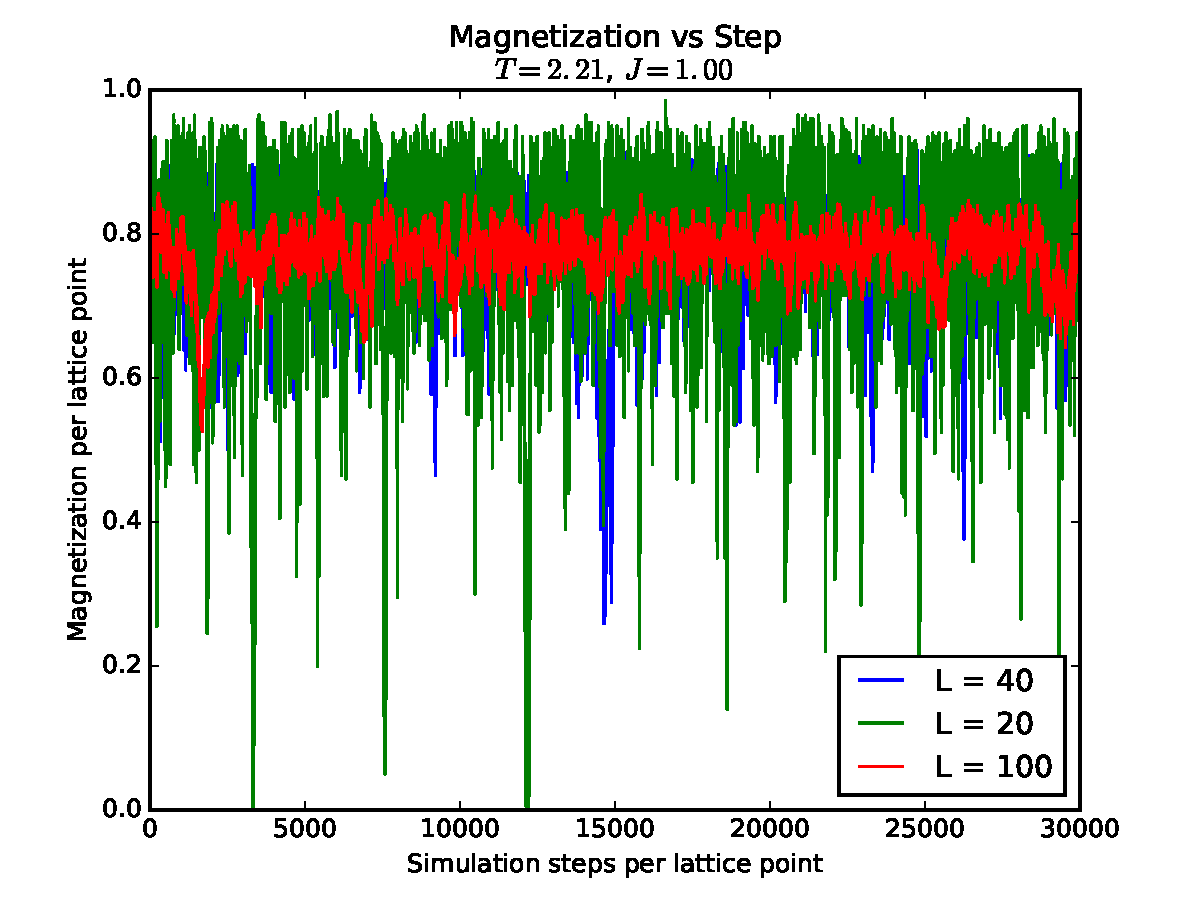
\includegraphics[width=0.4\textwidth]{{../graphs/MvsN-met}.pdf}
  \end{center}
  \caption{Plot of the magnetization per lattice point as a function of simulation steps per lattice point (sslp), using Metropolis algorithm.}
  \label{fig:AvsN-met}
\end{figure}

In figure \ref{fig:AvsN-met} we can easily see a thermalization time of around 100 sslp, however, as we could expect it depends heavily on $T$. In this simulation we are starting from a system with uniform spins, equivalent to a system at exactly $T=0$, and thus the system equilibrates quicker at $T=2.1$ (as shown in the plot) than at $T=10$, after the phase transition. Later on we will take a second look at this.

\begin{figure}[H]
  \begin{center}
    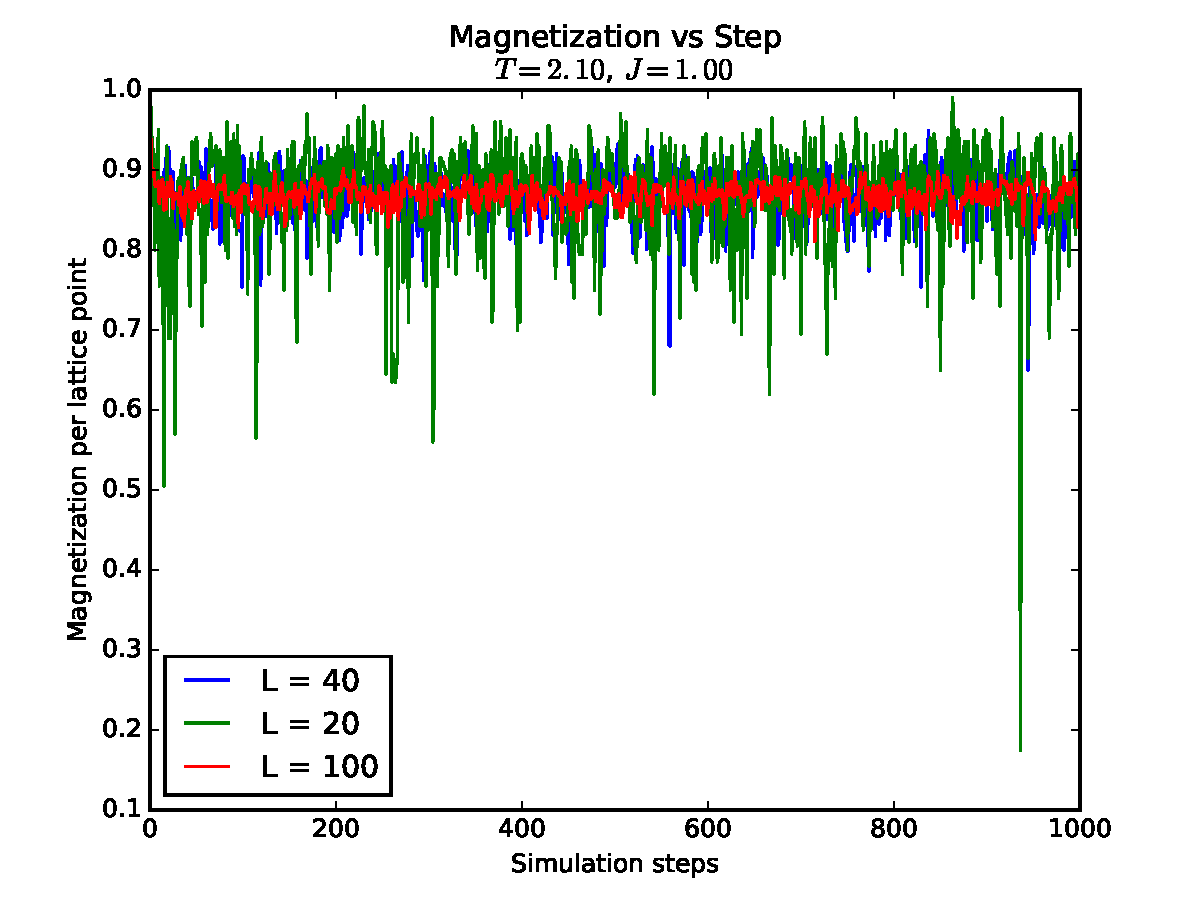
\includegraphics[width=0.4\textwidth]{{../graphs/MvsN-wolff}.pdf}
  \end{center}
  \caption{Plot of the magnetization per lattice point as a function of simulation steps, using Wolff's algorithm.}
  \label{fig:AvsN-wolff}
\end{figure}

In figure \ref{fig:AvsN-wolff} we can see a similar plot using the Wolff algorithm. Of course, this algorithm provides significantly lower correlation times, as we will see later it's around 10 to 20 simulation steps. Plotting the energy as a function of steps would gives a similar result, so we can omit the explicit plot. There is a better way to compute how much time should we wait, and it involves computing what is called autocorrelation function. We can compute this both using the energy or the magnetization, using the following expression

\begin{equation} \label{eq:autocorrelation} \begin{matrix} \xi_M(t) =  & \frac{1}{t_{\text{max}} - t} \sum_{t'=0}^{t_{\text{max}}-t} M(t')M(t'+t) \\
             & - \frac{1}{t_{\text{max}} - t} \sum_{t'=0}^{t_{\text{max}}-t} M(t') \\
             & \times \frac{1}{t_{\text{max}} - t} \sum_{t'=0}^{t_{\text{max}}-t} M(t'+t) \end{matrix} \text{ .} \end{equation}

And equivalently for the energy. From $\xi(t)$ we can compute the correlation time $\tau$ as

\begin{equation} \label{eq:corrtime} \tau = \frac{1}{\xi(0)} \int_0^\infty \dif t \xi(t) \text{ ,} ~~~~ \xi(0) = \avg{M^2} - \avg{|M|}^2 \text{ ,}  \end{equation}

where we could change $M(t)$ by $E(t)$ and do the same with the energy. Firstly, using equation (\ref{eq:autocorrelation}) we find the following results, using the Metropolis algorithm, for energy:

\begin{figure}[H]
  \begin{center}
    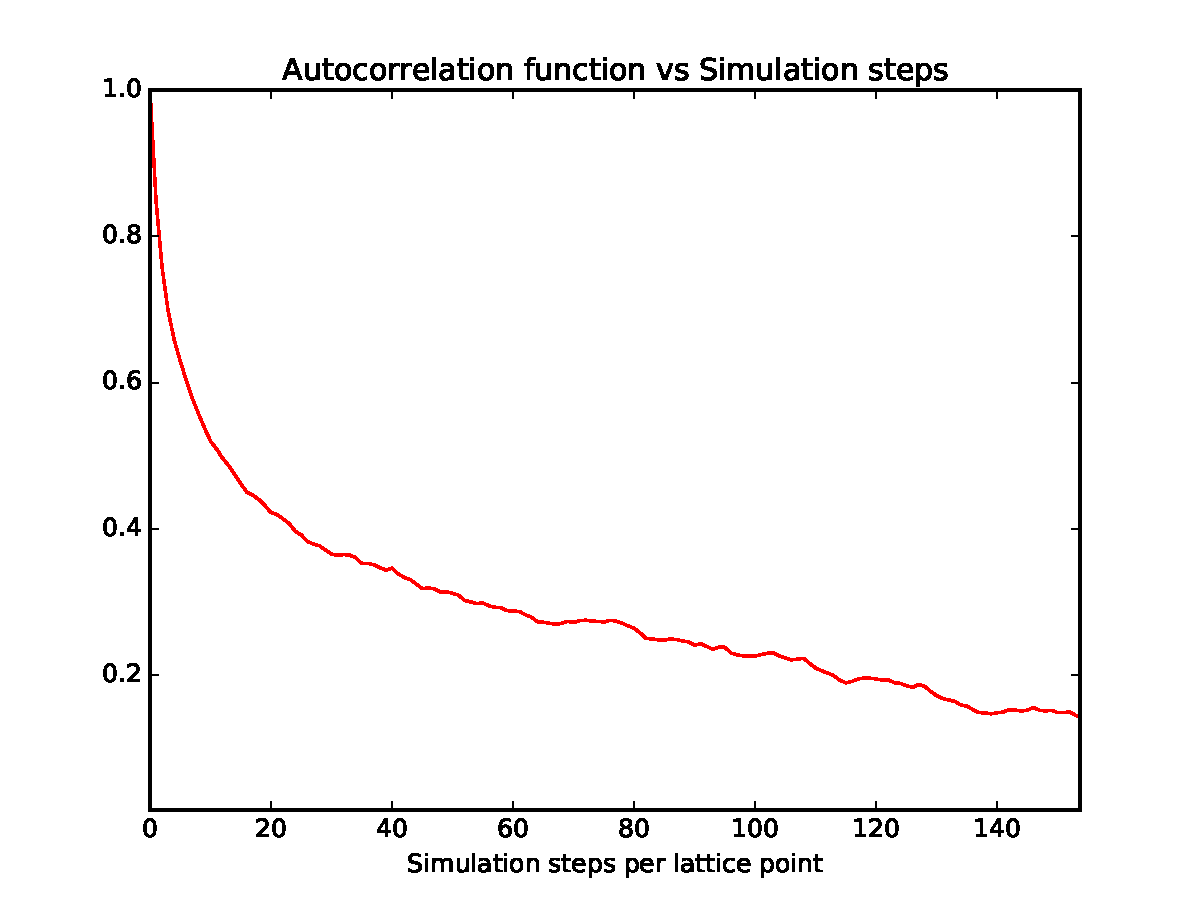
\includegraphics[width=0.45\textwidth]{{../graphs/AvsN-E-met}.pdf}
  \end{center}
  \caption{Plot of the autocorrelation function $\xi_E(N)$.}
\end{figure}

From here we can already estimate the correlation time, by looking at how much time does it take to go from one to $e^{-1}$, and we see that it's around one hundred or so time steps. Computing the autocorrelation function using the magnetization provides us with slightly similar results:

\begin{figure}[H]
  \begin{center}
    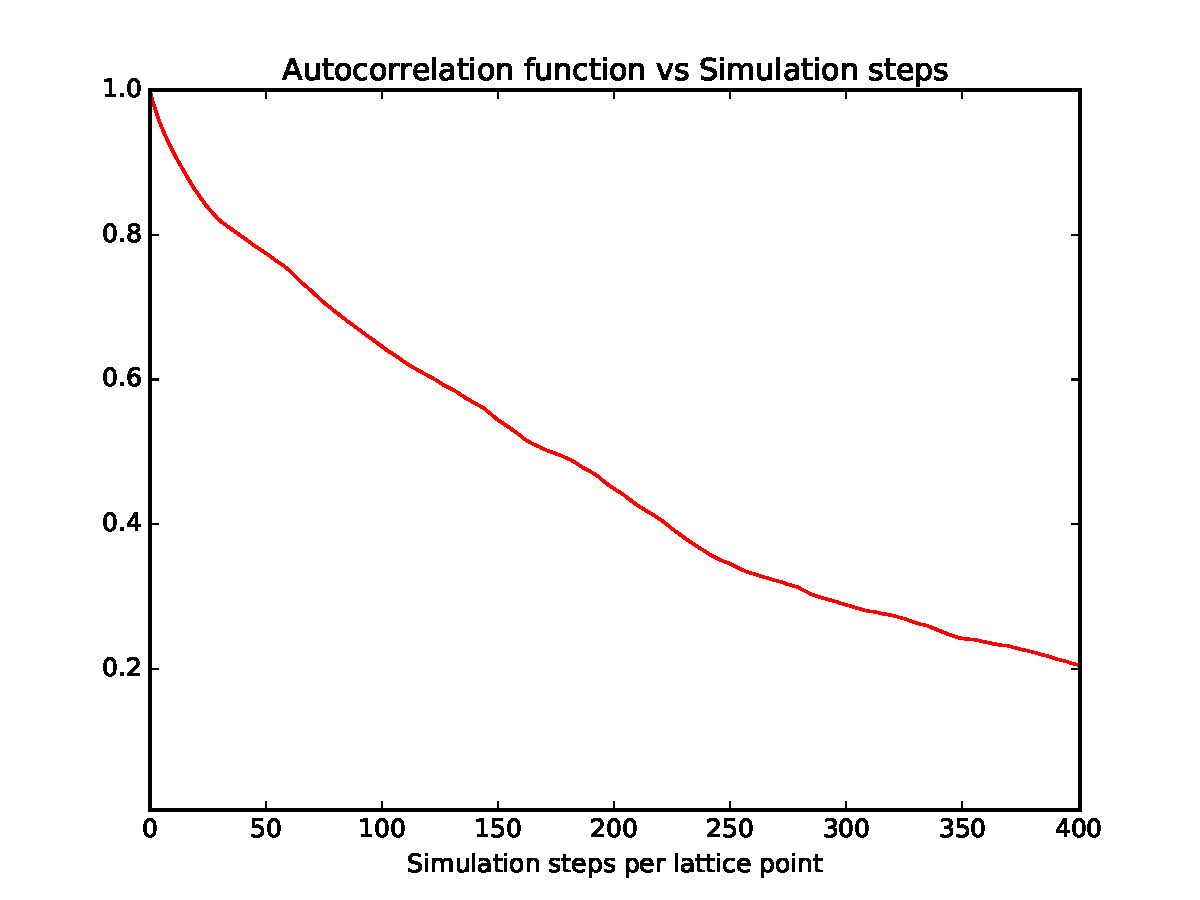
\includegraphics[width=0.45\textwidth]{{../graphs/AvsN-M-met}.pdf}
  \end{center}
  \caption{Plot of the autocorrelation function $\xi_M(N)$.}
\end{figure}

Remarkably, the correlation time for magnetization is slightly larger than for the energy. This small difference won't change our results, though, as we will always be simulating the system over several tenths of thousands steps, and thus we will have enough different system configurations to get precise enough results. Moreover, because of the way the energy and magnetization are computed, there are other factors that lead to more precision when measuring magnetization-related quantities.

However, using equation (\ref{eq:corrtime}) gives a much better result that we can plot as a function of $T$, and thus giving us a better understanding of its behavior. In the following plot we can see $\tau(T)$ for the Metropolis algorithm.

\begin{figure}[H]
  \begin{center}
    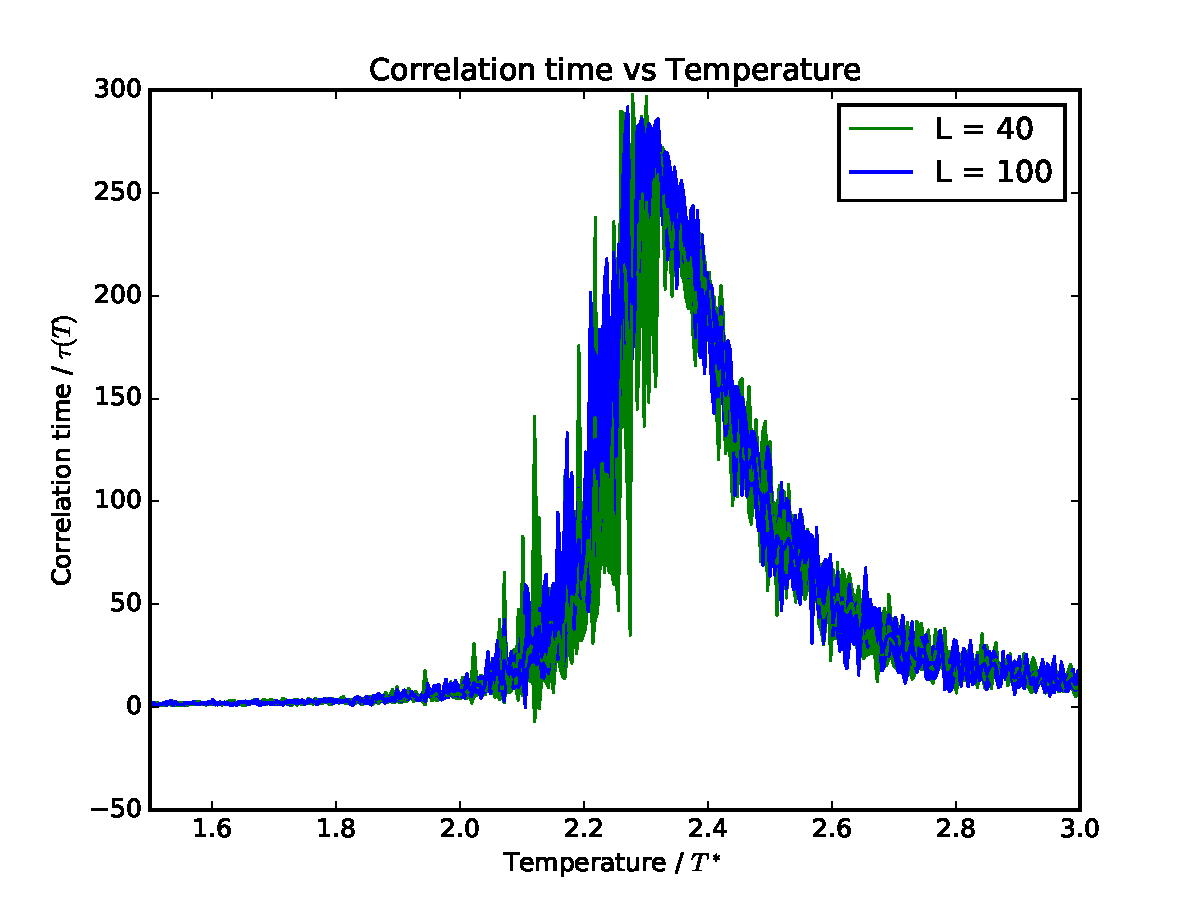
\includegraphics[width=0.45\textwidth]{{../graphs/TauvsT-met}.pdf}
  \end{center}
  \caption{Plot of the correlation time $\tau(T)$ using magnetization for the Metropolis algorithm. In this plot we have used error bands instead of bars, showing that within our precision it doesn't depend on the system size.}
\end{figure}

We can see that near the critical point the correlation time is significantly larger than anywhere else, due to the nature of the algorithm. Because of that, precise simulations near the critical point will take a long time when using the Metropolis algorithm. However, repeating this procedure for the Wolff algorithm we find significantly lower correlation times, meaning this algorithm generates statistically different configurations quicker than Metropolis', and therefore simulations give better results.

\begin{figure}[H]
  \begin{center}
    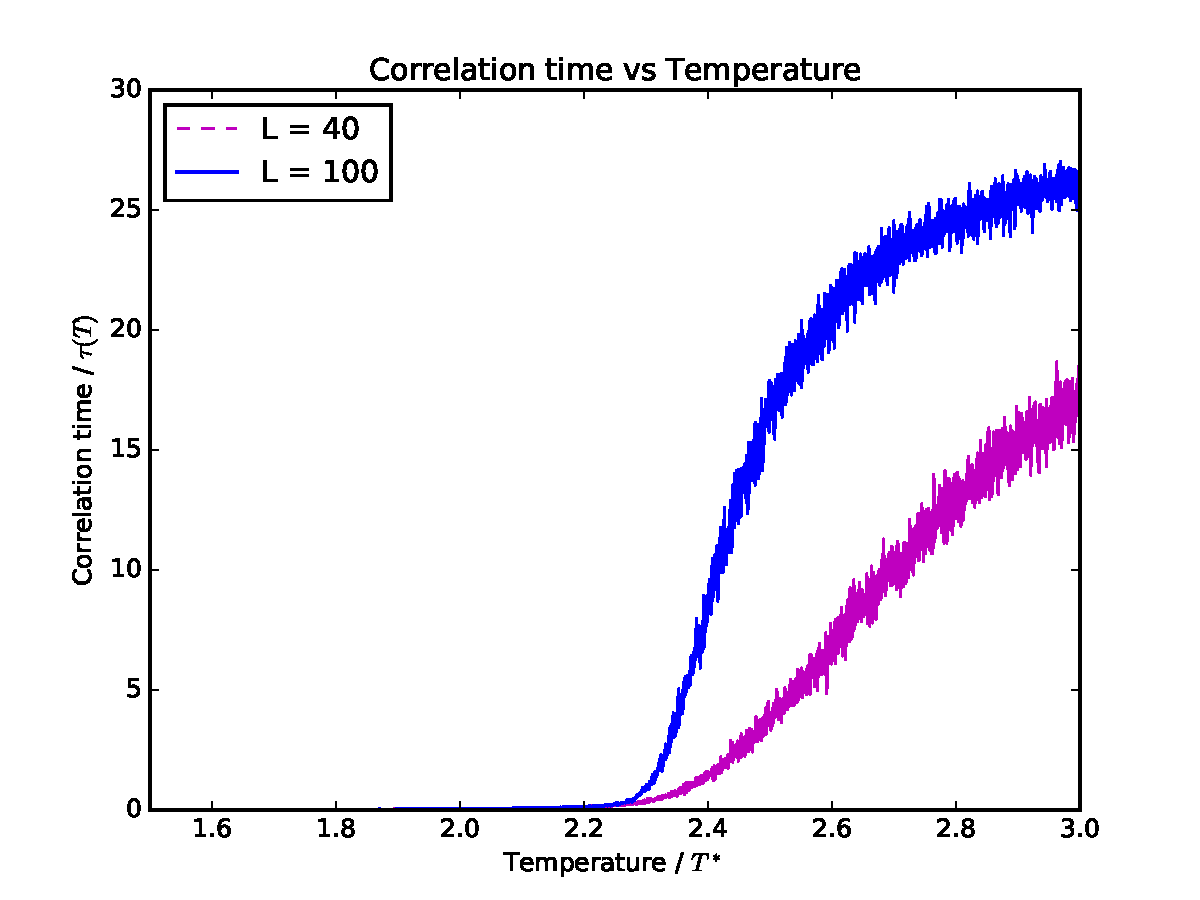
\includegraphics[width=0.4\textwidth]{{../graphs/TauvsT-wolff}.pdf}
  \end{center}
  \caption{Plot of the correlation time $\tau(T)$ using magnetization for the Wolff algorithm.}
\end{figure}

Using Wolff's algorithm we find a completely different dependence, specially for $T>T_c$. Of course, because of the way this algorithm works (adding spins to clusters) it's going to have a hard time trying to generate different system configurations when there are no spin domains in the system anymore. Therefore, for simulations in this regime the Metropolis algorithm is way more efficient. It's also worth mentioning that now we do see system size effects affecting the correlation time, however only for $T>T_c$, $\tau$ being higher for larger values of $L$.

\subsection{A remark about statistical errors}

As everything in physics, we need to estimate how good is a measurement, and for that we will follow the bootstrap method. This means that, on every plot of some quantity $X(T)$ that depends on temperature, we will compute statistical errors using

\begin{equation}
  \sigma(X) = \sqrt{\avg{X^2(T)}-\avg{X(T)}^2} \text{ ,}
\end{equation}

where the average is computed over several values obtained from a number of independent simulations. Because of the data density, error bars can be not so easy to see clearly, but will give us a general idea of how much our results vary from one simulation to the other.

\section{Phase transition}

Now that we have introduced all the core concepts implicitly used in every simulation, let's proceed to study some properties of the phase transition.

\subsection{Energy $E(T)$ and Magnetization $|M(T)|$}

We will start this section plotting both energy and magnetization as a function of temperature, where we would expect to see some sign of the phase transition. However, due to the nature of numerical simulations, points with infinite slope are not possible to reproduce, and thus to explicitly show the phase transition we are required to follow other procedures.

\begin{figure}[H]
  \begin{center}
    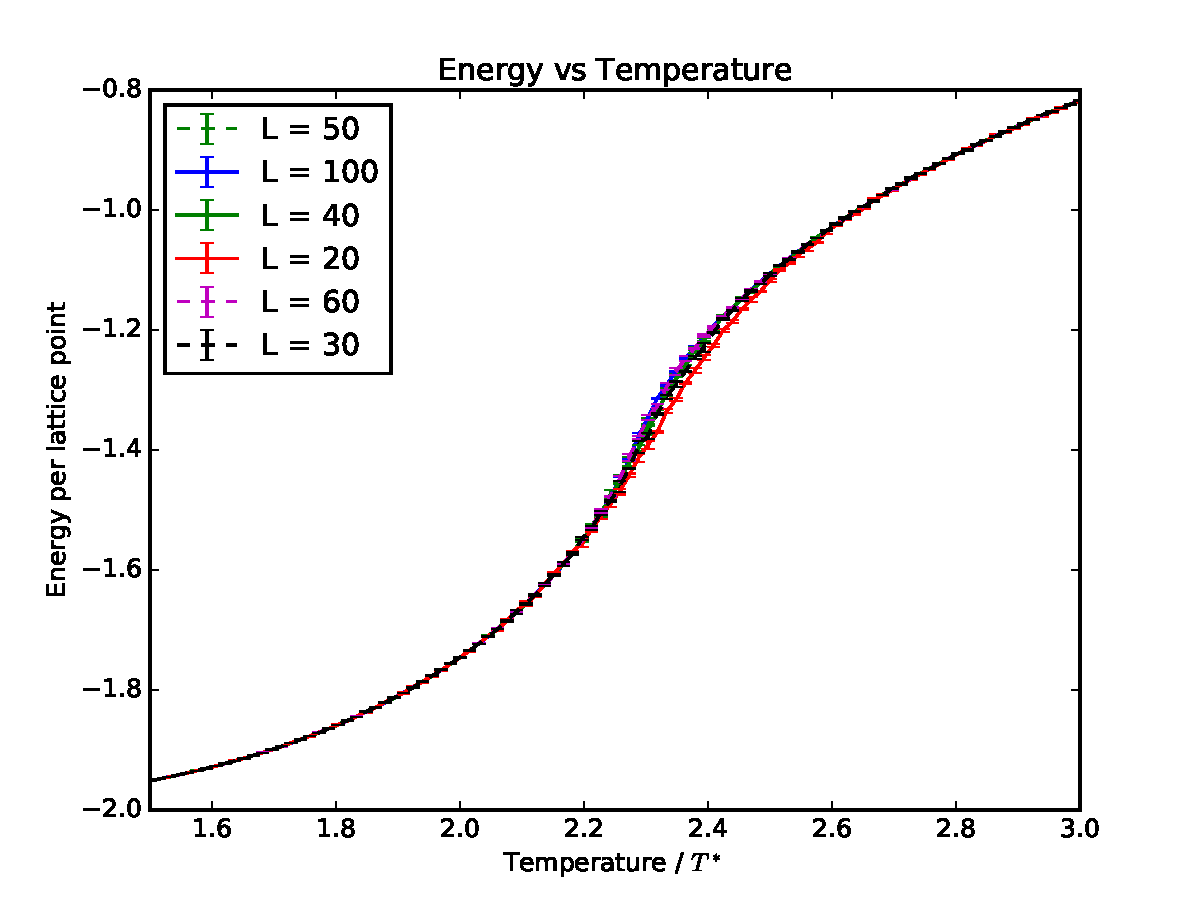
\includegraphics[width=0.4\textwidth]{{../graphs/EvsT-met}.pdf}
  \end{center}
  \caption{Plot of the energy of the system per lattice point for several values of temperature, averaging after reaching equilibrium. Data generated using the Metropolis algorithm.}
  \label{fig:EvsT-met}
\end{figure}

Even if we don't see the critical point directly in figure \ref{fig:EvsT-met}, we can easily infer that it's going to be located around $T=2.25$, just by looking at the position of the inflexion point. However, the infinite slope behavior that theory predicts cannot be seen as we had expected.

\begin{figure}[H]
  \begin{center}
    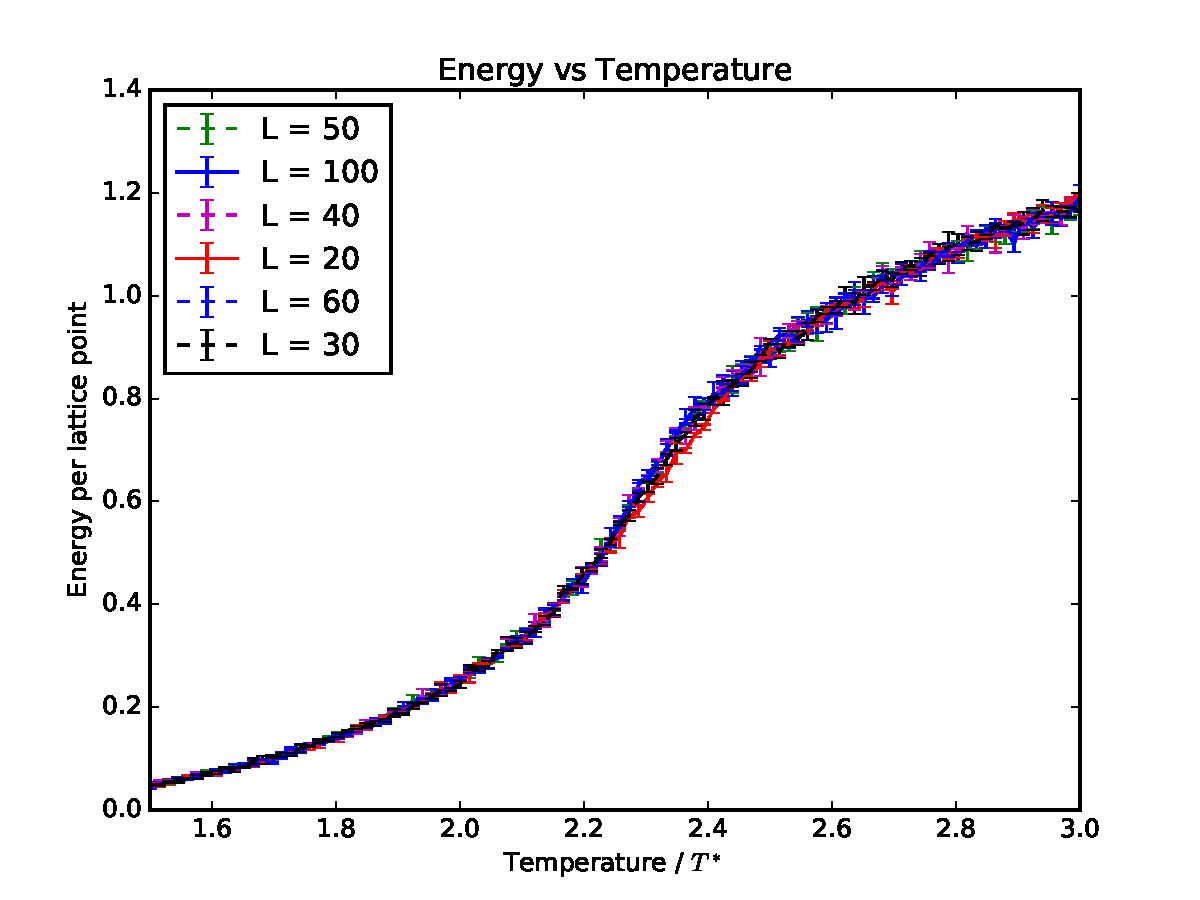
\includegraphics[width=0.4\textwidth]{{../graphs/EvsT-wolff}.pdf}
  \end{center}
  \caption{Plot of the energy of the system per lattice point for several values of temperature, averaging after reaching equilibrium. Data generated using the Wolff algorithm.}
  \label{fig:EvsT-wolff}
\end{figure}

 Now, comparing it to data from the Wolff algorithm from figure \ref{fig:EvsT-wolff} we find very similar results, except for a slightly larger error bars in Wolff's algorithm. As a general remark, the energy per lattice point does not depend on the system size, as we expect.

 We can compare these two figures to those of the magnetization, and since theory predicts a fairly specific behavior for $|M(T)|$ we can compare it to the analitical solution as well. First, in figure \ref{fig:MvsT-met} we can see results obtained using the Metropolis algorithm.

\begin{figure}[H]
  \begin{center}
    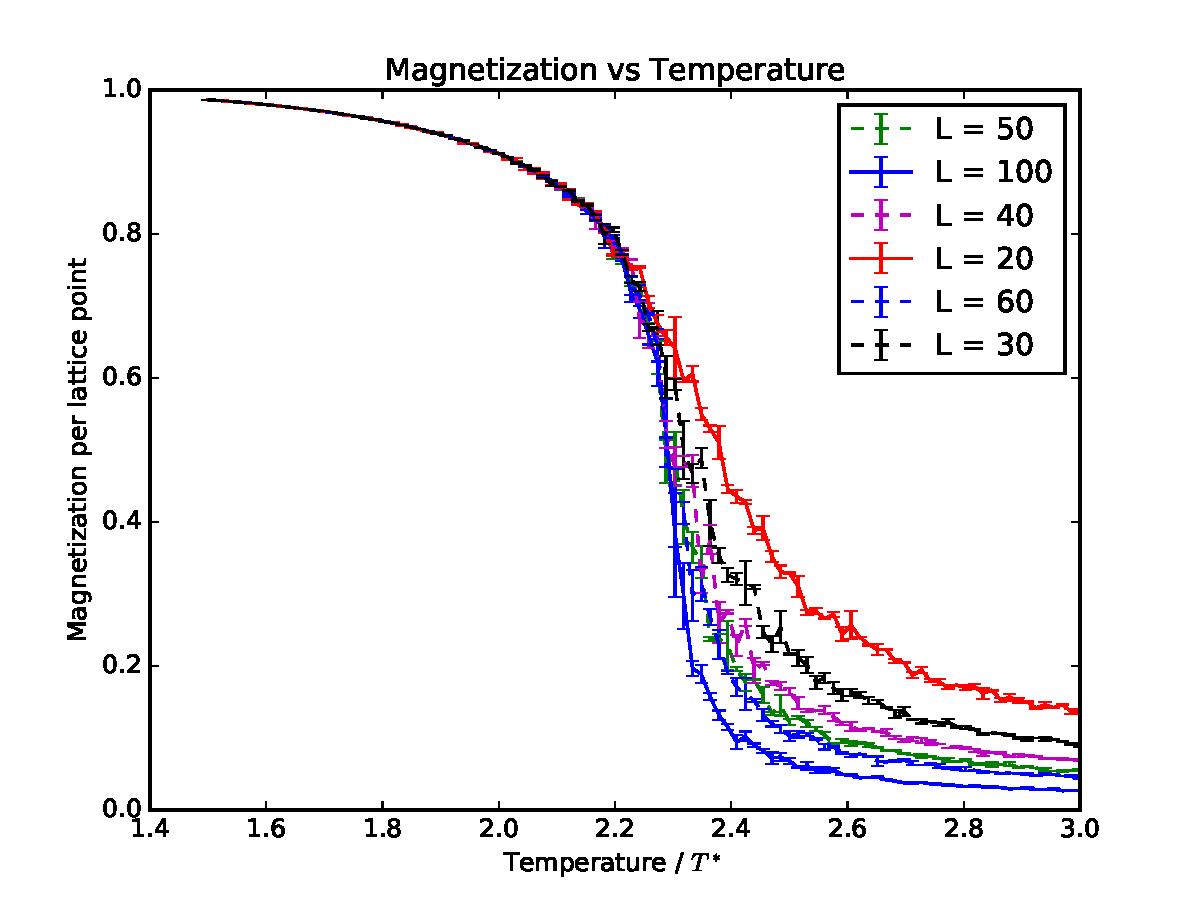
\includegraphics[width=0.4\textwidth]{{../graphs/MvsT-met}.pdf}
  \end{center}
  \caption{Plot of the magnetization of the system per lattice point for several values of temperature, averaging after reaching equilibrium. Data generated using the Metropolis algorithm.}
  \label{fig:MvsT-met}
\end{figure}

As opposed to the energy, in this case the error computing magnetization is significantly larger when using the Metropolis algorithm rather than the Wolff algorithm. This situation can be explained looking back at correlation times for both algorithms, since as we can see in the figure the largest error bars lie around the critical point. Since we are doing the same number of simulation steps per lattice point as cluster flips, the number of different configurations is significantly lower for the Metropolis algorithm. In figure \ref{fig:MvsT-wolff} we can see the equivalent plot using Wolff's algorithm data.

\begin{figure}[H]
  \begin{center}
    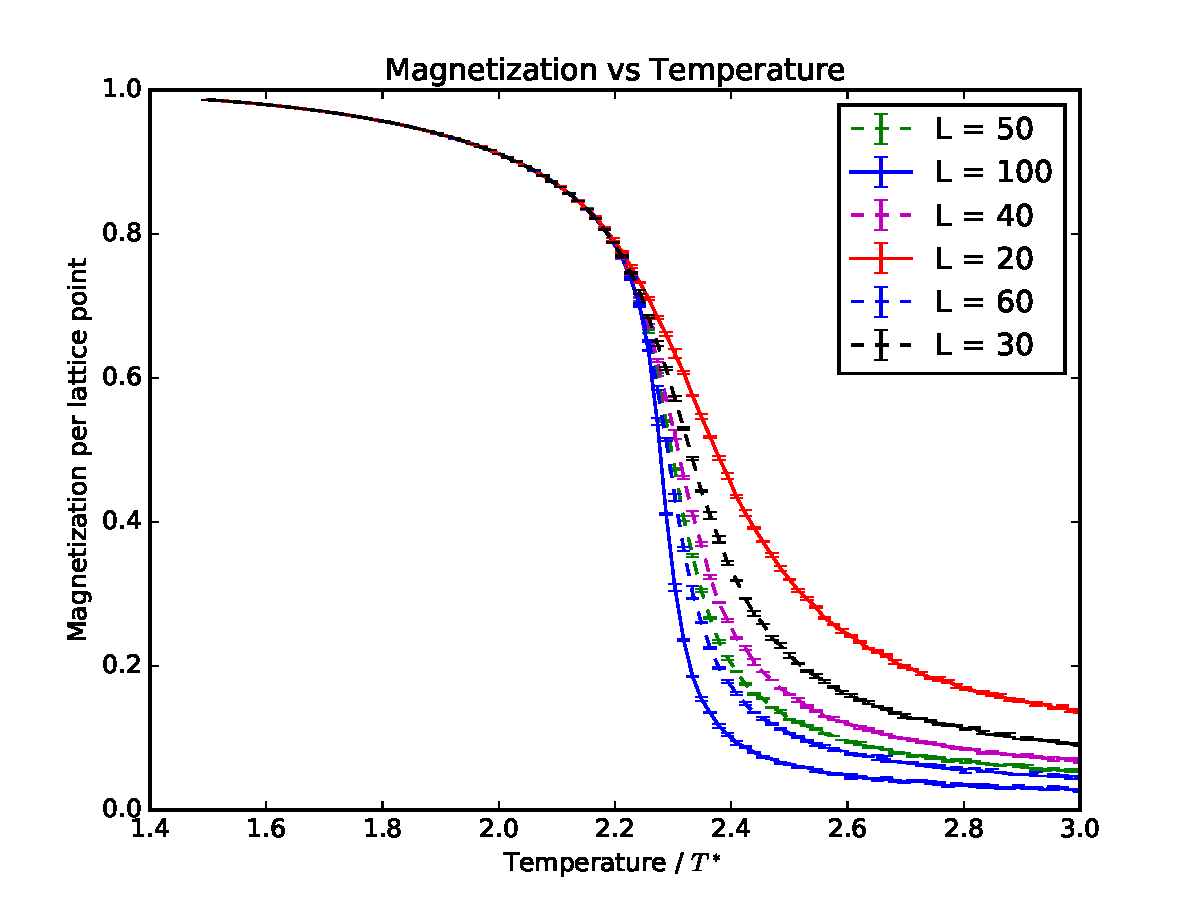
\includegraphics[width=0.4\textwidth]{{../graphs/MvsT-wolff}.pdf}
  \end{center}
  \caption{Plot of the magnetization of the system per lattice point for several values of temperature, averaging after reaching equilibrium. Data generated using the Wolff algorithm.}
  \label{fig:MvsT-wolff}
\end{figure}

Another significant remark in comparison with the energy, $M(T)$ does depend on the system size. These are boundary effects, which affect very differently how we compute these two quantities. Recall that we are computing the energy using equation (\ref{eq:hamiltonian}), while the magnetization is computed by

\begin{equation} M = \sum_i s_i \text{ .} \end{equation}

Since the energy is a more ``local'' quantity than magnetization, it will not be as affected as the latter by boundary conditions. However, even if in figure \ref{fig:MvsT-wolff} we cannot see the expected behavior predicted by theory, it's clear that for $L\rightarrow\infty$ we would recover it, and the inflexion point again marks where the critical point is supposed to be, again around $T=2.25$.

\subsection{Specific Heat $c_s(T)$ and Magnetic Susceptibility $\chi(T)$}

After computing the energy and magnetization of the system, we can proceed to compute more involved quantities, that in the end will lead to compute the critical exponents. As before, we will compare results both coming from the Wolff algorithm and the Metropolis algorithm, and for different system sizes as well. Let's start with the specific heat $c_s(T)$, which is given by

\begin{equation}
  c_s = \frac{\beta^2}{N}(\avg{E^2}-\avg{E}^2) \text{ .}
\end{equation}

In figure \ref{fig:CvsT-met} we can see a plot of the results given by the Metropolis algorithm. Even though we don't have precise measurements near the critical point, we can infer a few general ideas from this plot. First, since $E(T)$ does not depend on the system size, we don't expect $c_s(T)$ to depend either as we can see, although this is not true for three dimensional systems. This behavior will significantly affect the critical exponent related to this quantity as we will see in the following section.

\begin{figure}[H]
  \begin{center}
    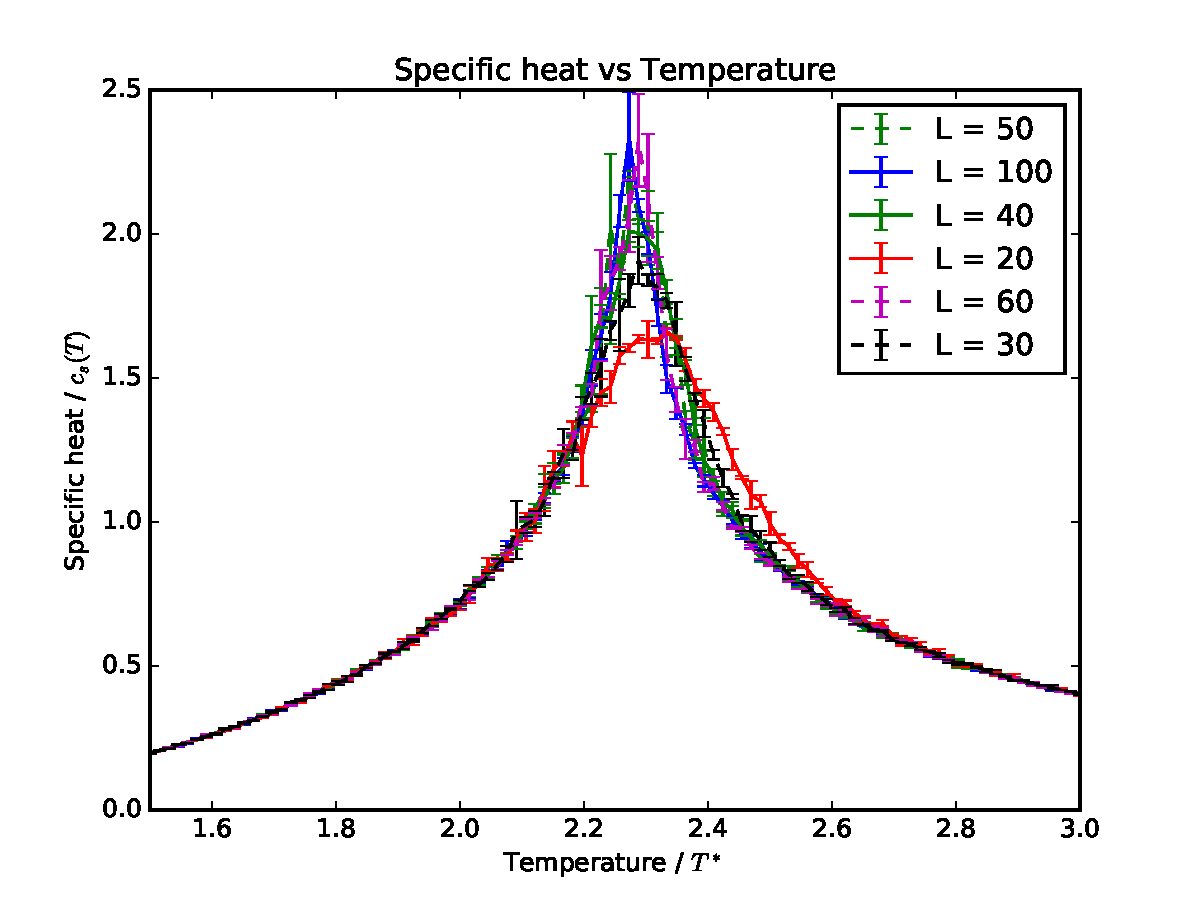
\includegraphics[width=0.4\textwidth]{{../graphs/CvsT-met}.pdf}
  \end{center}
  \caption{Plot of the specific heat of the system for several values of temperature, averaging after reaching equilibrium. Data generated using the Metropolis algorithm.}
  \label{fig:CvsT-met}
\end{figure}

It is also clear from these results where exactly is the critical point located, as we expected around $T=2.25$. In the next section we will calculate $T_c$ more precisely. A final remark, we can see that small fluctuations in $E(T)$, as shown in figure \ref{fig:EvsT-met} can lead to significant variations in derived data, and thus precise measurements are essential.

Let's continue analyzing the magnetic susceptibility $\chi(T)$ of the system, and comparing results coming from both algorithms. As before, in figure \ref{fig:XvsT-met} we can see our data computed with the Metropolis algorithm, and in figure \ref{fig:XvsT-wolff} the equivalent with the Wolff algorithm.

\begin{figure}[H]
  \begin{center}
    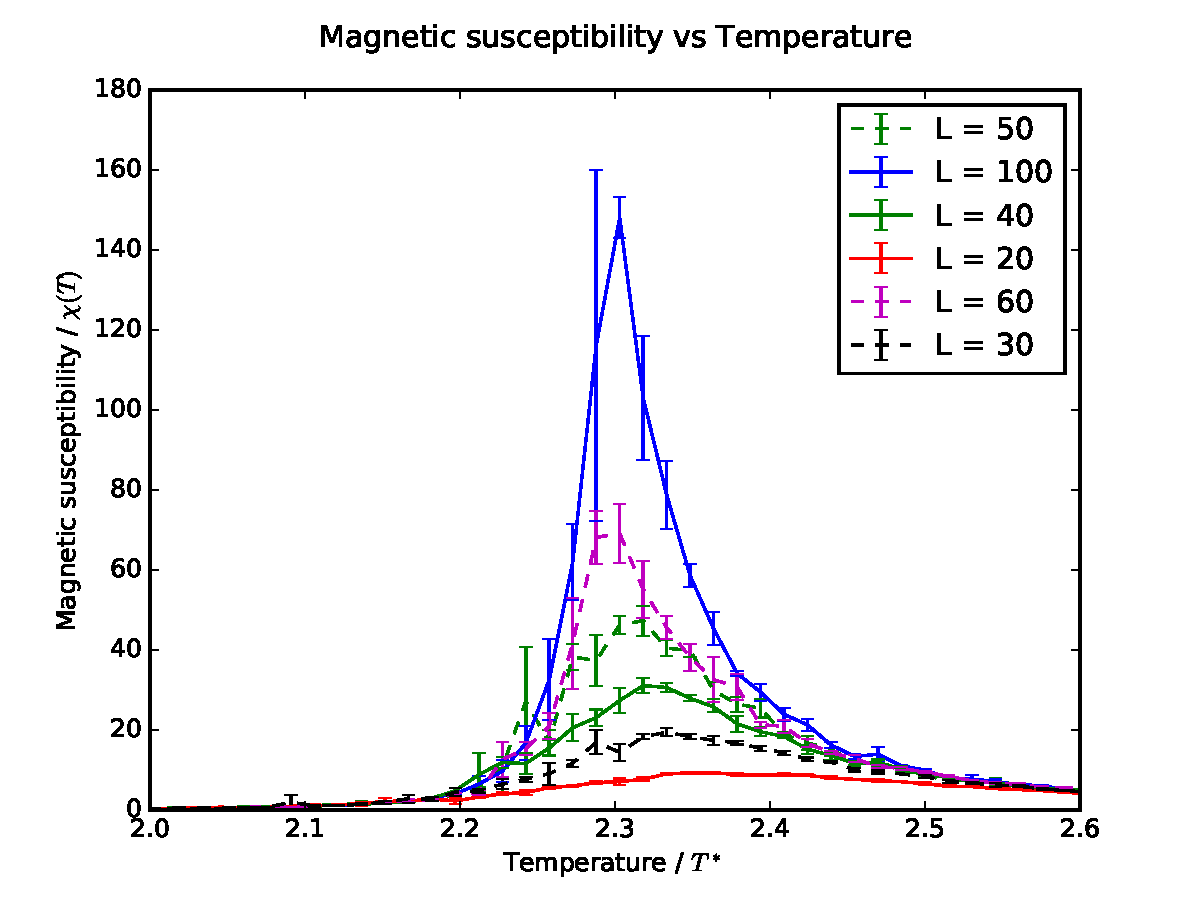
\includegraphics[width=0.4\textwidth]{{../graphs/XvsT-met}.pdf}
  \end{center}
  \caption{Plot of the magnetic susceptibility of the system for several values of temperature, averaging after reaching equilibrium. Data generated using the Metropolis algorithm.}
  \label{fig:XvsT-met}
\end{figure}

As we could have expected by looking at the plots of $|M(T)|$, the Metropolis algorithm gives way worse results than Wolff's, so to compute critical exponents we will be using mostly the latter. Since in the magnetization we found some system size dependence, we also expect to find some in these two plots, and as we can see, near the critical point $\chi(T_c)$ increases with $L$.

\begin{figure}[H]
  \begin{center}
    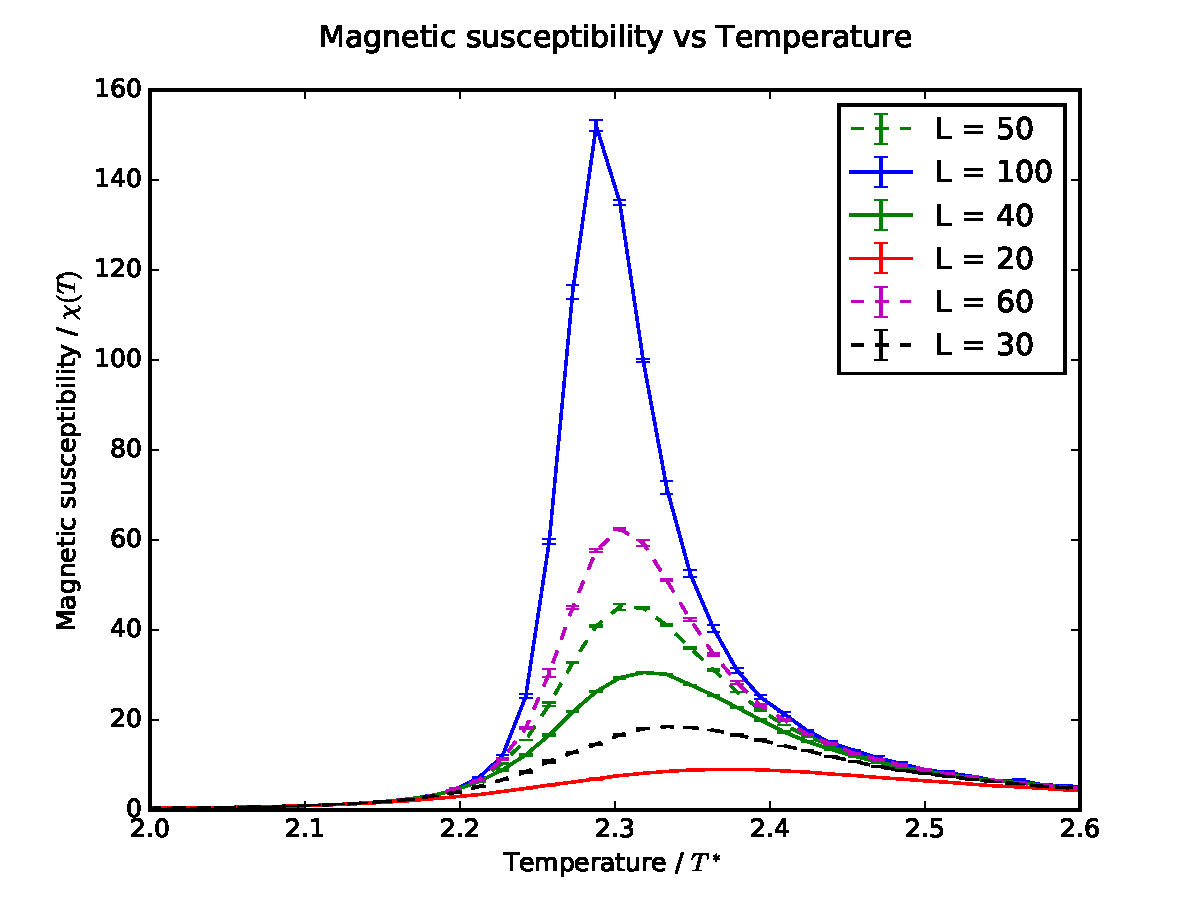
\includegraphics[width=0.4\textwidth]{{../graphs/XvsT-wolff}.pdf}
  \end{center}
  \caption{Plot of the magnetic susceptibility of the system for several values of temperature, averaging after reaching equilibrium. Data generated using the Wolff algorithm.}
  \label{fig:XvsT-wolff}
\end{figure}

\subsection{Critical point and critical exponents}

Let's finally proceed to compute the critical point and critical exponents. The method we are going to follow is known as data collapse, and consists on multiplying some quantity $X(T)$ by $L$ to some power. Now, by choosing the right values for the exponents, the dependence of the data with the system size should disappear, and thus become only one line. The exponents that satisfy this collapse are called critical exponents.

Besides the critical exponents, we are going to compute the critical point by transforming temperatures like the following

\begin{equation}
  t = \frac{T-T_c}{T_c} \text{ ,}
\end{equation}

and then multiply it by $L$ with some exponent. By correctly choosing the critical exponents and critical point we can do the data collapse. First, let's define the coefficients we are going to compute:

\begin{equation}
  \left\{
  \begin{matrix*}
    t & \rightarrow & L^{\frac{1}{\nu}}\\
    \chi(T) & \rightarrow & L^{-\frac{\gamma}{\nu}}\\
    c_s(T) & \rightarrow & L^{-\frac{\alpha}{\nu}}\\
  \end{matrix*}
  \right.
  \text{ .}
\end{equation}

We are going to compute them both in two and three dimensions, since this procedure doesn't change. Let's begin with $\chi(T)$. In practice, what we did to determine the best fit was to plot several combinations of values until we found the most appropriate. In the following plot we can see our results:

\begin{figure}[H]
  \begin{center}
    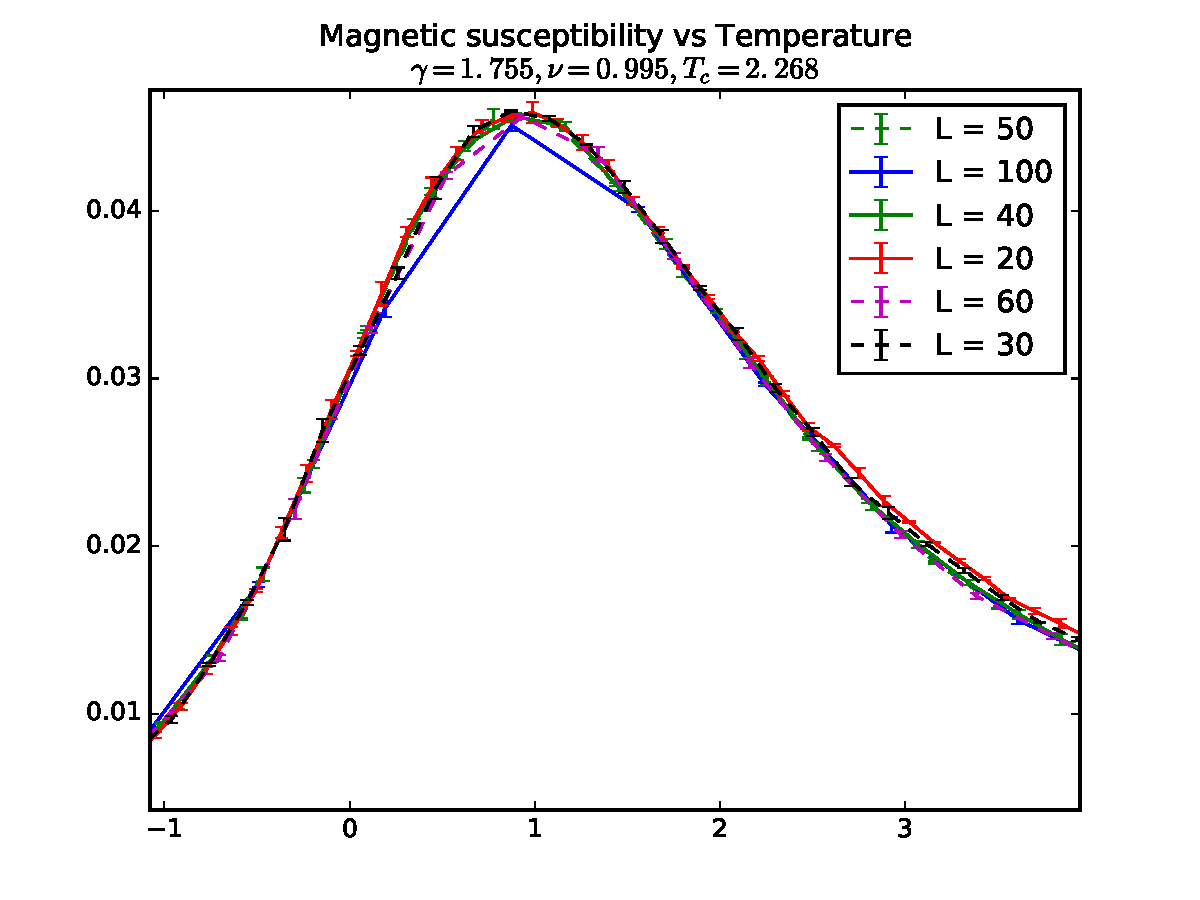
\includegraphics[width=0.4\textwidth]{{../graphs/XvsT-exp-2}.pdf}
  \end{center}
  \caption{Plot of $\chi(t L^{\frac{1}{\nu}})L^{-\frac{\gamma}{\nu}}$ for a two dimensional system. Values found: $\gamma = 1.755$, $\nu = 0.995$, $T_c=2.268$.}
  \label{fig:XvsT-exp-2}
\end{figure}

Since we are working with our best data, it's not a surprise that we can find $\gamma$ and $\nu$ with such accuracy. As we can see, all the lines collapse to the same one, as far as our precision goes, so we can say that these are precise enough values for the exponents. In the next figure we can see a similar result, but using a three dimensional system instead.

\begin{figure}[H]
  \begin{center}
    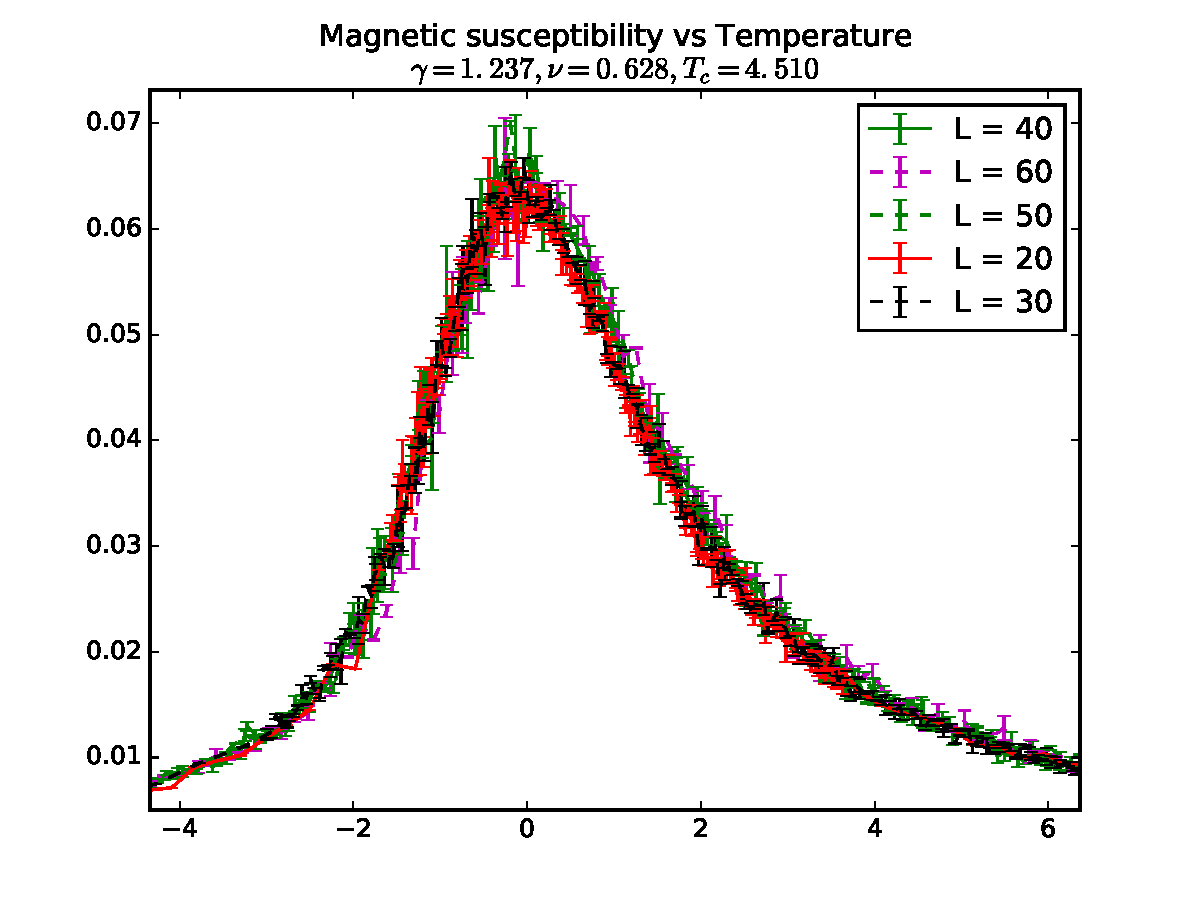
\includegraphics[width=0.4\textwidth]{{../graphs/XvsT-exp-3}.pdf}
  \end{center}
  \caption{Plot of $\chi(t L^{\frac{1}{\nu}})L^{-\frac{\gamma}{\nu}}$ for a three dimensional system. Values found: $\gamma = 1.237$, $\nu = 0.628$, $T_c=4.51$.}
  \label{fig:XvsT-exp-3}
\end{figure}

In this case we find significantly larger error bars, because of several reasons. First, the correlation time in a three dimensional system is slightly larger than in two dimensions, and therefore, to get the same amount of different system configurations we need to simulate over a larger amount of steps. However, in three dimensions $N$ grows as $L^3$, so computing each simulation step takes longer. In conclusion, our results are going to be less accurate unless we significantly increase simulation time.

Although, within our precision this is a good enough result, close to what other more accurate simulations find. It's worth noticing that $T_c$ is now higher than in the two dimensional case, while $\gamma$ and $\nu$ become lower.

Let's now compute $\alpha$ using the specific heat $c_s(T)$. Since we already know $T_c$ and $\nu$, $\alpha$ is the only parameter we are going to vary and fit. As before, the following plot contains the best fit we have found for a two dimensional system:

\begin{figure}[H]
  \begin{center}
    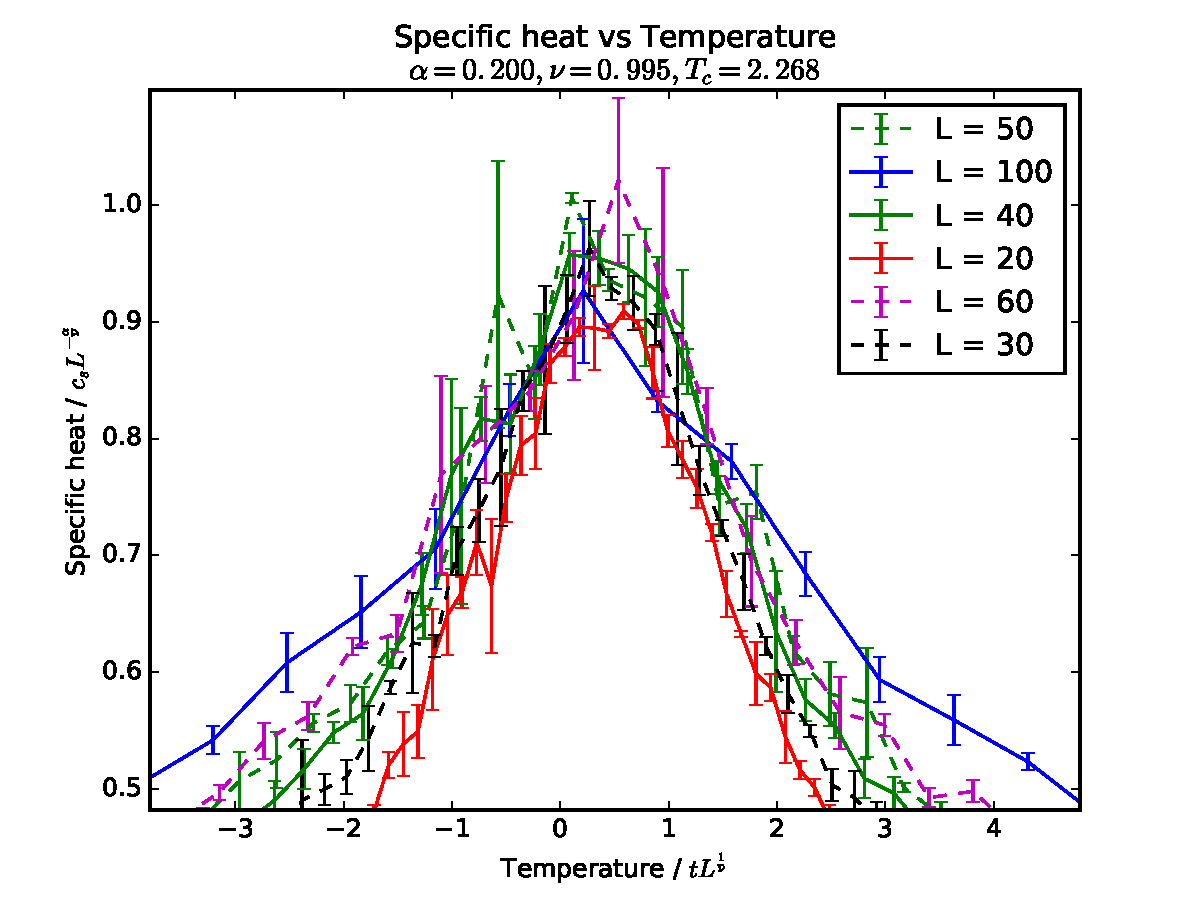
\includegraphics[width=0.4\textwidth]{{../graphs/CvsT-exp-met-2}.pdf}
  \end{center}
  \caption{Plot of $c_s(t L^{\frac{1}{\nu}})L^{-\frac{\alpha}{\nu}}$ for a two dimensional system. Values found: $\alpha \sim 0.2$.}
  \label{fig:CvsT-exp-2}
\end{figure}

As expected, these results are not as accurate as the ones before, mainly due to the fact that we have found more statistical fluctuations when computing $E(T)$ than with $\chi(T)$. However, theory predicts a value of $\alpha=0$, which we could have predicted by looking at figures \ref{fig:CvsT-met} and \ref{fig:EvsT-met}, since they should not depend on $L$, and thus the exponent of $L$ multiplying $c_s(T)$ should be zero. However, we find a value of $\alpha \sim 0.2$ which should have a large error margin because of these reasons.

In three dimensions we find:

\begin{figure}[H]
  \begin{center}
    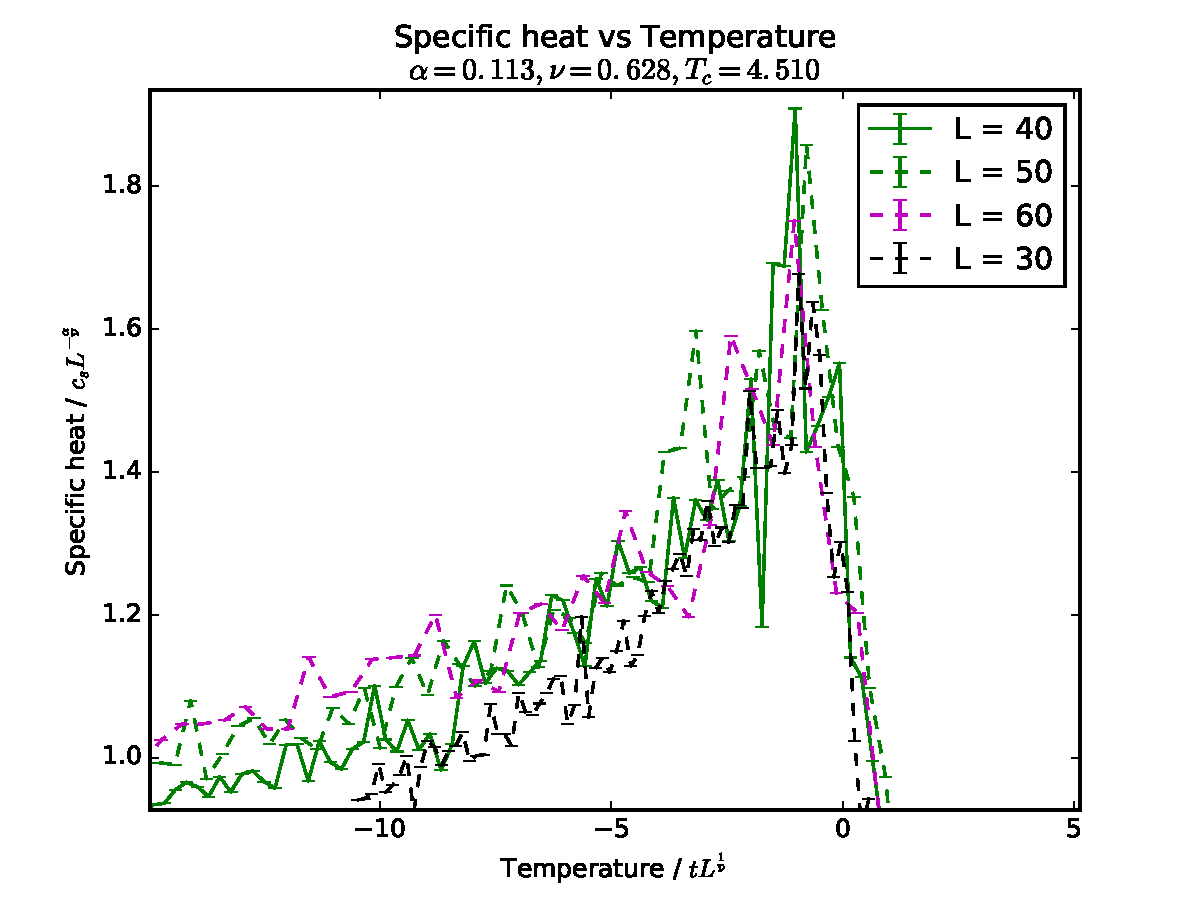
\includegraphics[width=0.4\textwidth]{{../graphs/CvsT-exp-met-3}.pdf}
  \end{center}
  \caption{Plot of $c_s(t L^{\frac{1}{\nu}})L^{-\frac{\alpha}{\nu}}$ for a two dimensional system. Values found: $\alpha \sim 0.11$.}
  \label{fig:CvsT-exp-3}
\end{figure}

As we could expect, the accuracy of these results is not quite good, however it is enough to determine that $\alpha \sim 0.1$ in three dimensions.

\section{Conclusions}

In this project we have implemented several algorithms to numerically solve the Ising model in different situations, ending up computing the critical exponents. There are many other extensions to this model that we could have studied, for example an external magnetic field $B\neq0$, other critical exponents, or more algorithms.

After analyzing our results we can conclude that we have successfully determined the critical exponents, as well as understood at a deeper level the dynamics of the Ising model.

\end{document}
